\section{Evaluation Methodology}
\subsection{Implementation}
We prototype and evaluate \systemname on a Huawei Smartwatch 2 wearable device. The smartwatch is equipped with a Quad-core Cortex-A7
processor at 1.1 GHz.  It runs Android Wear 2.0 operating system. We use \FIXME{four} sensors provided by the smartwatch: the
accelerometer, gyro, and \FIXME{xx}. The collected sensor data are sent via Bluetooth to a XiaoMI Note2 Android smartphone for
post-processing and event detection. 

\begin{figure}[!thbp]
	\centering
	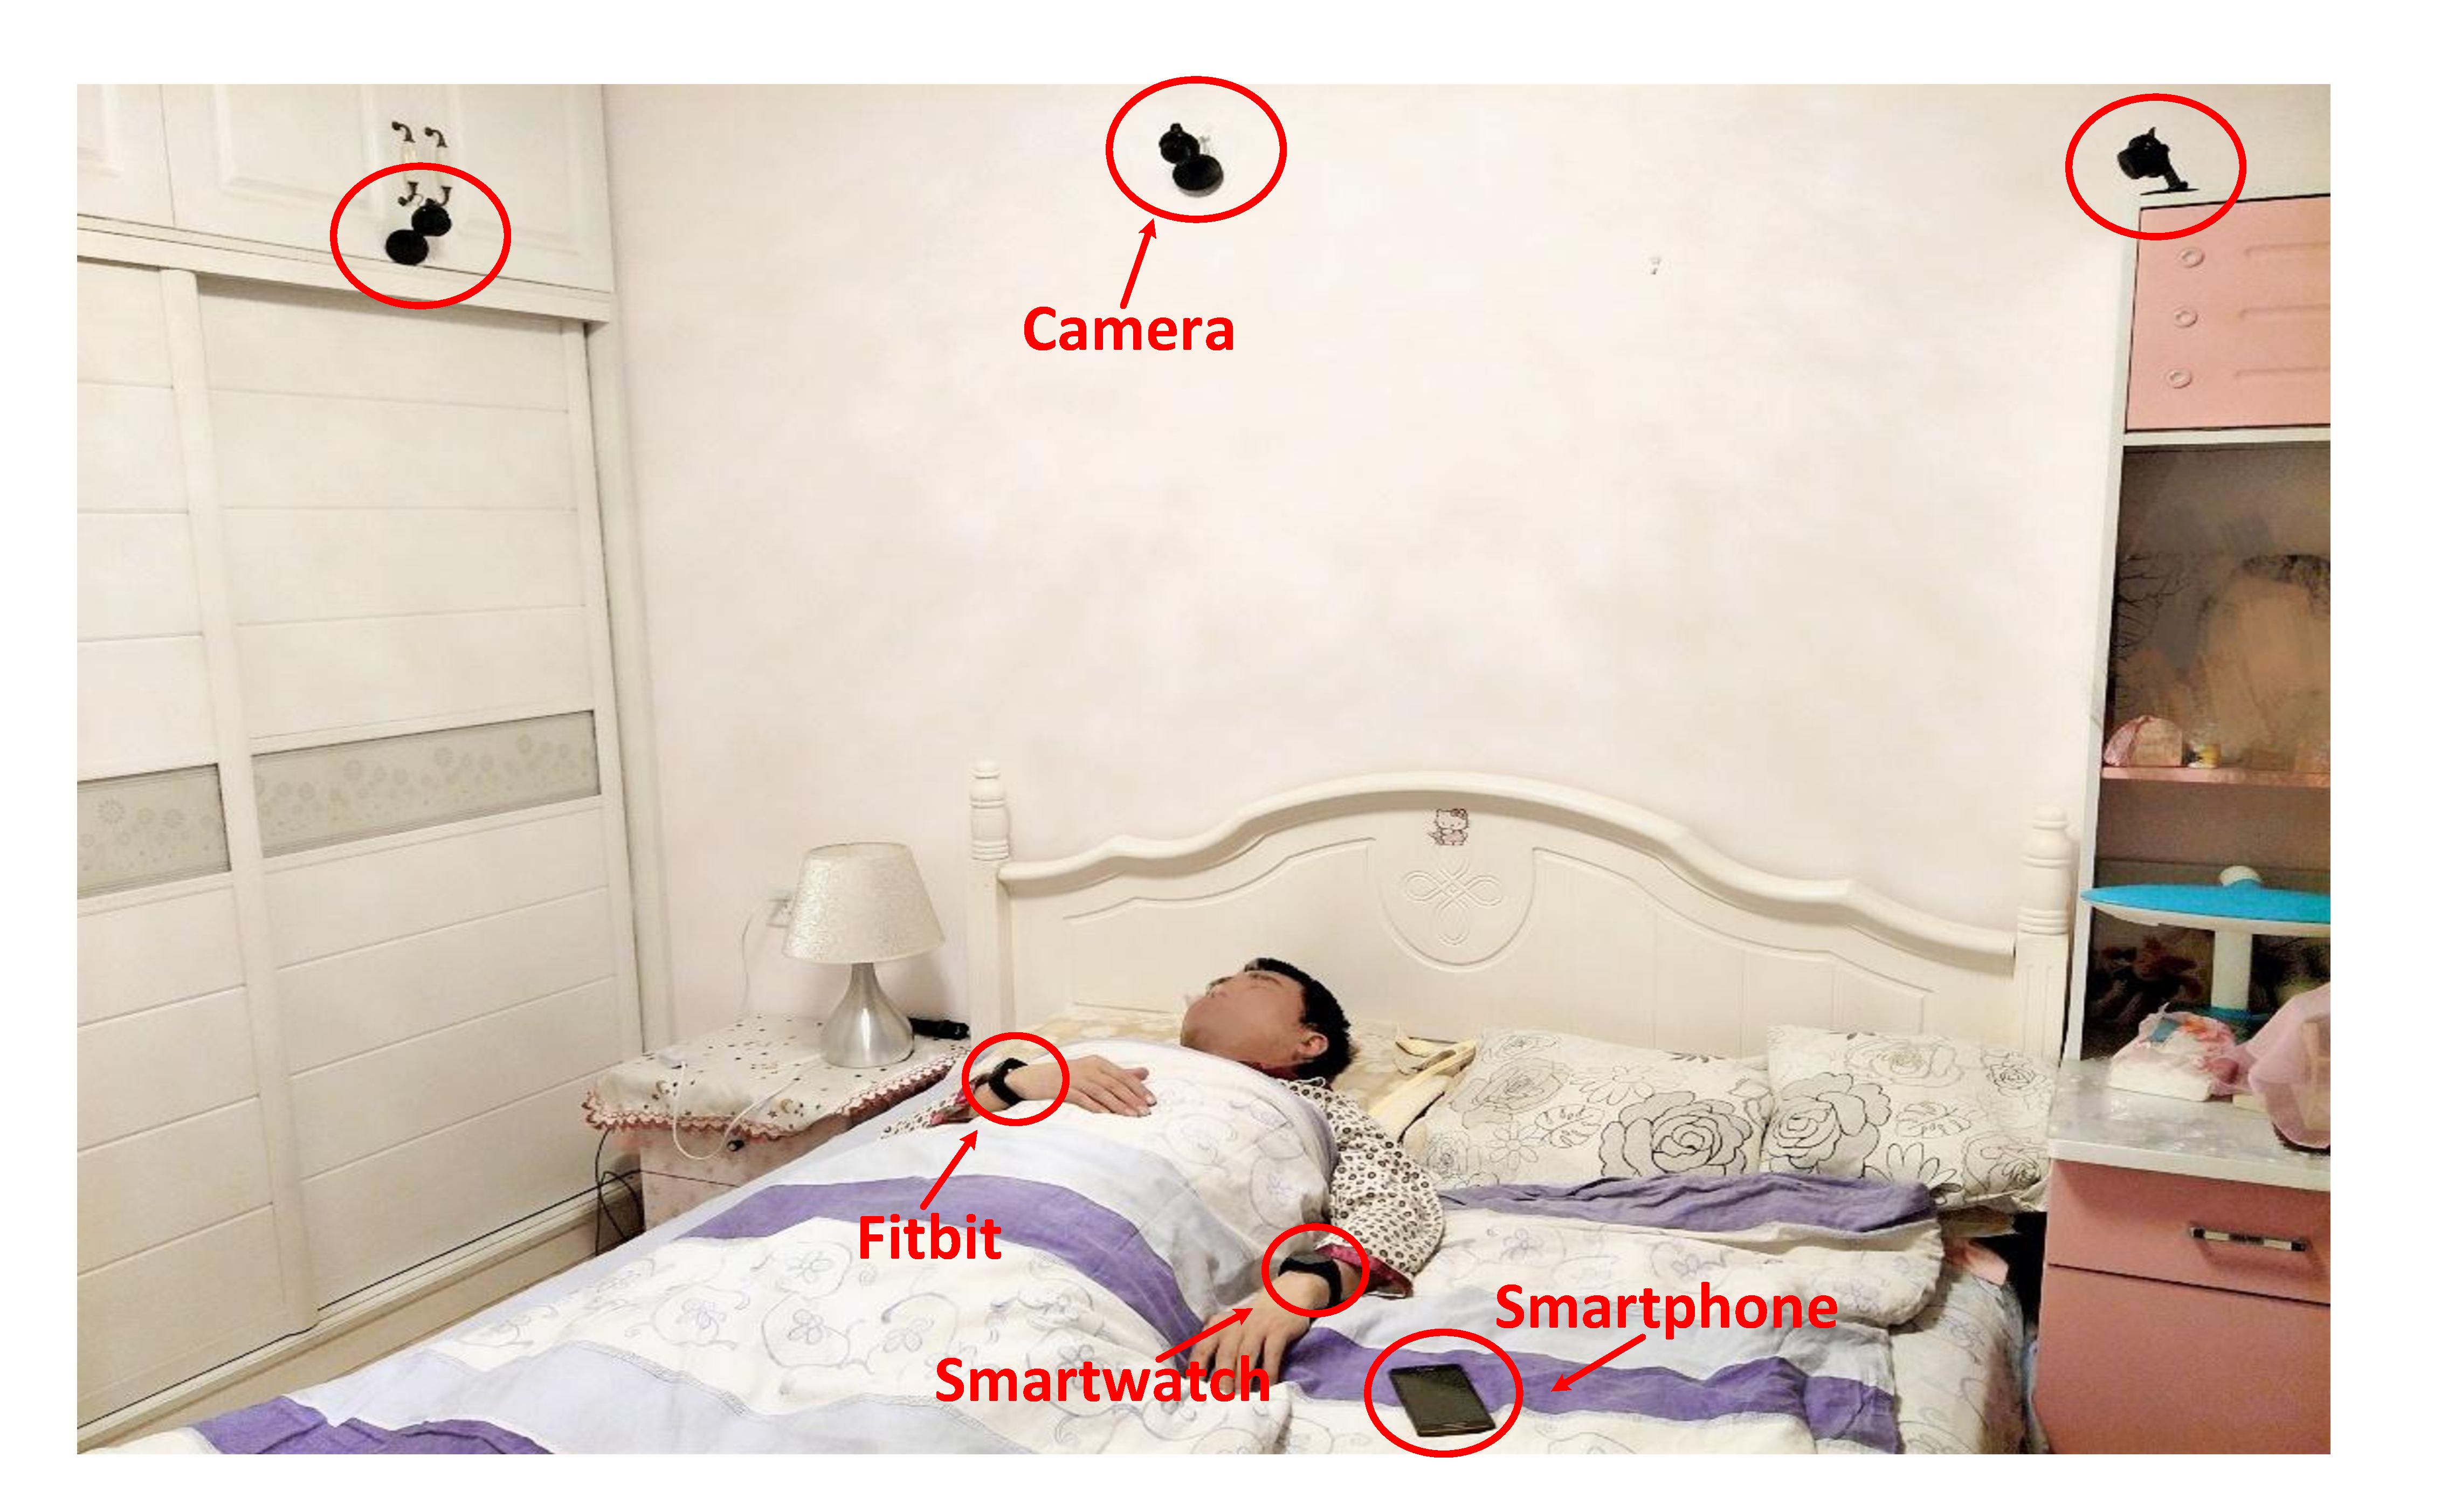
\includegraphics[width=0.52\linewidth]{Figures/setup.pdf}
	\caption{Deployment setup.}\label{fig:setup}
\end{figure}

\FIXME{ZW: here we should detail our experimental setup e.g. the environmental settings, how do we recruit the users, the mixture of the
users, what are the competitive models that we compare with, how do we report data (e.g. do we apply any statistical methods to remove the
outliers?), etc.}
=======
%\section{Experimental Setup} {\systemname} is implemented on the HuaWei Smartwatch 2. The programming platform is JAVA. For simplification,
%we implement the event detection on a laptop and the collected data is processed by MATLAB. \textcolor{blue}{In our experiments, we recruit
%15 volunteers (6 males and 9 females) from 15 years old to 60 years old,  of whom 5 people are between the ages of 15 and 25, and 5 are
%between the ages of 25 and 40, and 6 people between 40 and 60 years old. According to our preliminary survey of participants, two of 40 to
%60 year old are found to have long-term sleep disorders,  one with difficulty falling asleep and having a light sleep with more dreams, and
%another participant with the symptoms of awaking at night and early awakening, and there is a 53-year-old participant have been troubled by
%snoring, they are the focus of our attention. In addition, other participants occasionally suffer some sleep problems such as insomnia,
%snore and so on.} The experiments are conducted over two weeks, and during experiments, these volunteers sleep alone in a quiet room and
%each of them sleeps at least 6 hours. Moreover, each participant is asked to wear a smartwatch and Fitbit Charge2 \cite{fitbit} on his/her
%wrist simultaneously during sleep. And the smartphone with Sleep As Android \cite{SleepAndroid} is placed beside the participant's body.
%Considering that there is no absolute ground truth to detect sleep stage and the operations of other professional medical equipment are
%complicated, we leverage the result of Fitbit Charge2, a comfortable and effortless bracelet, as the ground truth. Sleep As Android, a
%widely used app for sleep detection, run the whole sleep process for comparing with our system. At the same time, to test the reliability
%of our methods, we use the video camera to monitor the sleep, and those recorded data by camera are set as groundtruth during the
%experiment. \textcolor{red}{Fig.00000} illustrates the experimental scene for our system.



\subsection{User Participation} We have recruited 15 volunteers to participate in our experiments. Our
participants include 6 males and 9 females at the age of between 15 and 60 years old. Two of our participants have been diagnosed with
long-term, on-going sleep-related disorders, and one participant has described that his sleep is significantly affected by snoring. These
three participants are our focus group.

\subsection{Experimental Setup}
After obtaining IRB approval, we have conducted our experiments over a two-week period. During experiments, these volunteers sleep alone in
a quiet room and each of them sleeps at least 6 hours. Moreover, each participant is asked to wear a smartwatch and Fitbit Charge2
\cite{fitbit} on his/her wrist simultaneously during sleep. And the smartphone with Sleep As Android \cite{SleepAndroid} is placed beside
the participant's body. Considering that there is no absolute ground truth to detect sleep stage and the operations of other professional
medical equipment are complicated, we leverage the result of Fitbit Charge2, a comfortable and effortless bracelet, as the ground truth.
Sleep As Android, a widely used app for sleep detection, run the whole sleep process for comparing with our system. At the same time, to
test the reliability of our methods, we use the video camera to monitor the sleep, and those recorded data by camera are set as ground
truth during the experiment. \textcolor{red}{Fig.00000} illustrates the experimental scene for our system.

\FIXME{ZW: I will come back to this experimental setup section later.}
>>>>>>> 9a36d8509284f43467e34744950ae8fa1edec9aa
